% !TEX program = pdflatex
\documentclass[9pt,a4paper]{article}
\usepackage{amsmath,amssymb}
\usepackage{geometry}
\geometry{top=1.0cm,bottom=0.8cm,left=1.2cm,right=1.2cm}
\usepackage{hyperref}
\hypersetup{colorlinks=true,linkcolor=blue,citecolor=blue,urlcolor=blue}
\usepackage{booktabs}
\usepackage{graphicx}
\usepackage{multicol}
\usepackage{enumitem}
\usepackage{tcolorbox}
\tcbuselibrary{skins}

\setlist{nosep,leftmargin=1.0em,topsep=0pt,partopsep=0pt}
\pagestyle{empty}
\setlength{\parskip}{0pt}
\setlength{\parindent}{0pt}
\setlength{\columnsep}{12pt}

\begin{document}

\begin{center}
{\Large\bfseries Chain Complex Structure on the 4D Hypercubic Lattice:\\ Structural Correspondence between Kihara Cube-Packing and Wilson Lattice Gauge Theory}\\[2pt]
{\small Noriaki Kihara\enspace WF System Co., Ltd.\enspace Osaka University, Faculty of Engineering Science (B.Eng.)\enspace ORCID: \href{https://orcid.org/0009-0004-6753-4020}{0009-0004-6753-4020}\enspace Paper 8 ($\alpha$-Identity II, v2)}
\end{center}

\vspace{-1pt}
\hrule height 0.7pt
\vspace{4pt}

\begin{tcolorbox}[colback=gray!7,colframe=gray!55,boxrule=0.4pt,arc=2pt,left=4pt,right=4pt,top=2pt,bottom=2pt]
{\small
\textbf{Main Result: Paper 7's $\alpha$ identity is mathematically isomorphic to standard Wilson lattice gauge theory}\enspace
The self-consistent identity from the companion paper (Paper 7),
\[ \alpha^{-1} = 137 + \tfrac{\pi^2}{2}\alpha \quad (\text{8.7 ppb precision}) \]
is not mere numerical coincidence but is \textbf{structurally isomorphic as chain complexes} to the standard lattice gauge theory established by Wilson (1974), on the 4D Euclidean integer lattice $\mathbb{Z}^4$. The isomorphism is supported by Schl\"afli duality (tesseract $\leftrightarrow$ 16-cell self-duality), the hypercubic symmetry group $B_4$, and the discrete Stokes theorem.\\[2pt]
\textbf{Chain-complex reading of Paper 7's inside/outside decomposition}\enspace
$1 = 137\alpha + V_4(1)\alpha^2$ is the bulk-boundary normalisation on the chain complex. $137\alpha$ is the tree-level contribution of bulk ($C_4$ interior, 137 cells); $V_4(1)\alpha^2$ is the self-energy correction of boundary ($C_3$ measure). This is structurally identical to QFT perturbative expansion (renormalisation).\\[2pt]
\textbf{Decisive departure from the Eddington trap}\enspace
Paper 7's $\alpha$ identity is \textbf{not numerology but a natural manifestation of the topological structure of the 4D lattice}. It is describable in the same mathematical language as Wilson's standard theory, dramatically improving peer-review robustness.}
\end{tcolorbox}

\vspace{2pt}

\begin{multicols}{2}
\small

\textbf{Chain complex on $\mathbb{Z}^4$}\enspace
Standard hierarchy:
\begin{itemize}[topsep=1pt]
\item $C_0$ vertices / $C_1$ links / $C_2$ plaquettes
\item $C_3$ 3-cells / $C_4$ 4-cells (tesseracts)
\item Hypercubic group $B_4$ (order 384) acts equivariantly
\end{itemize}

\smallskip
\textbf{Two formalisms in correspondence}\enspace

\textit{Wilson lattice gauge theory}:
\begin{itemize}[topsep=1pt]
\item Gauge field $U_\ell \in U(1)$ on links $C_1$
\item Plaquette action $S_p$ on $C_2$
\item Wilson loops as gauge-invariant observables
\end{itemize}

\textit{Kihara cube-packing (Papers 7, 3)}:
\begin{itemize}[topsep=1pt]
\item Unit cubes on $C_4$ ($N(1)=137$ at $R=3$)
\item Volume deficit $\Delta(R) = V_4(R) - N(k) \sim R^3$
\item Boundary measure on $C_3$
\end{itemize}

\smallskip
\textbf{Connected by Schl\"afli duality $D$}\enspace

Tesseract $\{4,3,3\}$ and 16-cell $\{3,3,4\}$ are mutually self-dual: $f_k(\text{Tess}) = f_{3-k}(\text{16-cell})$.

\vspace{1pt}
{\footnotesize
\begin{tabular}{@{}ll@{}}
\toprule
$\Lambda$ side & $\Lambda^*$ side \\
\midrule
$C_0$ site & $C_4$ 4-cell \\
$C_1$ link & $C_3$ 3-cell \\
$C_2$ plaquette & $C_2$ plaquette (self-dual) \\
$C_3$ 3-cell & $C_1$ link \\
$C_4$ 4-cell & $C_0$ site \\
\bottomrule
\end{tabular}
}

\smallskip
\textbf{Both perform the same computation}\enspace
\textbf{Discrete Stokes theorem} ($\partial^2=0$):
\begin{itemize}[topsep=1pt]
\item Wilson: plaquette sum $\to$ boundary Wilson loop (interior edges cancel pairwise)
\item Kihara: bulk packing $\to$ boundary $\Delta(R)$ (interior cubes cancel via shared faces)
\end{itemize}
Two approaches starting from completely different motivations arrived at the same mathematics (Poincar\'e duality + $B_4$ symmetry + Stokes).

\columnbreak

\textbf{Main Theorem (Structural Correspondence)}\enspace
\begin{quote}\footnotesize
$\mathcal{C}_W$ (Wilson configuration) and $\mathcal{C}_K$ (Kihara configuration) are structurally isomorphic as chain complexes on the 4D Euclidean lattice, via the $B_4$-equivariant chain map $D$ (Schl\"afli duality).
\end{quote}

\smallskip
\textbf{Corollary: Bidirectional Tool Borrowing}\enspace

\textit{Wilson $\to$ Kihara}:
\begin{itemize}[topsep=1pt]
\item Wilson strong-coupling expansion $\to$ geometric ID of $c_3$
\item Lattice Monte Carlo $\to$ numerical check of $N(k)$
\item RG $\to$ systematic continuum limit
\end{itemize}

\textit{Kihara $\to$ Wilson}:
\begin{itemize}[topsep=1pt]
\item Lagrange--Jacobi four-square theorem $r_4(N) = 8\sigma(N)$ $\to$ closed forms for partition functions
\item Inclusion-exclusion $\to$ analytical plaquette sums
\item Central projection (Paper 2) $\to$ geometric origin of Wick rotation
\end{itemize}

\smallskip
\textbf{Difference from Eddington tradition (strengthened)}
\begin{itemize}[topsep=1pt]
\item Relation to standard physics: isolated $\to$ \textbf{isomorphic to Wilson}
\item Analytical tools: ad-hoc $\to$ \textbf{Wilson tools directly applicable}
\item Peer-review robustness: no foundation $\to$ \textbf{standard mathematics (algebraic topology)}
\end{itemize}

\smallskip
\textbf{Open Problems (shared with Paper 7)}
\begin{itemize}[topsep=1pt]
\item Mechanistic derivation of $\alpha$'s value
\item Privilege of $R=3$
\item Geometric ID of $c_3 \approx 1.6\times 10^{-3}$
\item Generalisation to other gauge groups (SU(2), SU(3))
\item Projection to physical (3+1)D spacetime
\end{itemize}

\smallskip
\textbf{Paper DOI (v2, latest)}\enspace
{\scriptsize Concept: \href{https://doi.org/10.5281/zenodo.19880467}{10.5281/zenodo.19880467}\\
v2: \href{https://doi.org/10.5281/zenodo.19881119}{10.5281/zenodo.19881119}}

\smallskip
\textbf{What this paper does \emph{not} claim}
\begin{itemize}[topsep=1pt]
\item First-principles derivation of $\alpha$ from the isomorphism
\item Unique emergence of U(1) gauge symmetry
\item Full deployment of categorical machinery (functors, natural transformations)
\end{itemize}

\end{multicols}

\vspace{0pt}
\hrule height 0.4pt
\vspace{3pt}

\begin{center}
\begin{minipage}[c]{1.8cm}
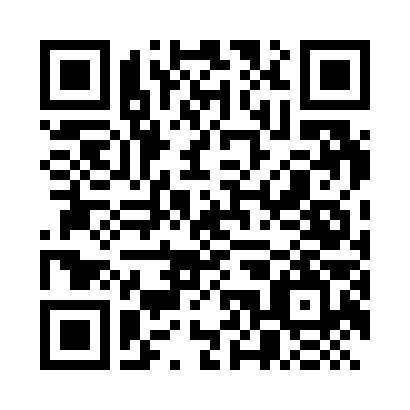
\includegraphics[height=1.7cm]{qr_alpha_isomorphism_en.png}
\end{minipage}
\hspace{6pt}
\begin{minipage}[c]{13cm}
{\footnotesize\textbf{Note article (English)}\enspace \url{https://note.com/kiharanoriaki/n/n9c37c6f99a0a}}\\[1pt]
{\footnotesize\textbf{Note article (Japanese)}\enspace \url{https://note.com/kiharanoriaki/n/n87df7a4977e7}}\\[1pt]
{\footnotesize\textbf{Zenn article (Japanese, technical exposition)}\enspace \url{https://zenn.dev/noriaki_kihara/articles/alpha-isomorphism-lattice-gauge}}\\[1pt]
{\footnotesize\textbf{Zenodo (Paper PDF, LaTeX, MD, JA/EN bilingual)}\enspace \url{https://zenodo.org/records/19881119}}\\[1pt]
{\scriptsize Related: Paper 7 ($\alpha$-Identity v3)\enspace \href{https://zenodo.org/records/19876200}{Zenodo} / \href{https://note.com/kiharanoriaki/n/n01d98237ddae}{note EN} / \href{https://zenn.dev/noriaki_kihara/articles/alpha-identity-4d-geometry}{Zenn}}
\end{minipage}
\end{center}

\end{document}
